\chapter{气候系统模式不确定参数优化方法设计}
\label{tu:tune}
\section{气候系统模式不确定参数优化问题}

上一章描述了气候系统模式中存在大量的不确定参数,这些参数对气候系统模式的模拟性能有很大的影响,进而影响了预测的准确率。优化算法是一种量化不确定性,校准不确定参数的有效方法。接下来将叙述在气候系统模式不断发展过程中遇到的各种不确定参数优化问题。

气候系统模式中存在一些重要的单一变量,比如降水,它对深对流,云物理等参数化方案中的不确定参数非常敏感。在单一的降水预报时为了提高预测能力需要针对降水对不确定参数进行校准。Yang B等人在中尺度天气预报模型WRF(Weather Research and Forecasting Model)中利用MVFSA(multiple very fast simulated annealing)方法对深对流中的不确定性参数做了校准~\cite{yang2015calibration}。

衡量一个气候系统模式整体性能的时候,通常会将多个变量综合在一起,形成一个较为全面的性能指标,在这个性能指标下优化模型的不确定参数。张涛等人将GAMIL( Grid-point Atmospheric Model of IAP LASG)大气模式中受到关注最多的变量综合成一个用来衡量模式平均态的综合性能指标,并利用改进的单纯形下山方法对GAMIL大气模式中对流和云等参数化方案中的不确定参数进行了调整~\cite{zhang2015automatic}。

上述问题都可以用单目标优化问题来描述,但是在气候系统模式参数优化中多目标优化也不可或缺。例如当模式预报的目标有两个以上,比如降水、温度和湿度等对预测十分重要的变量都需要尽可能得到优化,如果使用上述将多个变量综合成一个目标的方法,则有可能会出现整体的性能得到提升,但其中某个关键变量却变得很差的情况。此时需要利用多目标优化来对不确定参数进行校准。另外在气候系统模式中有很多非常重要的气候现象,例如热带大气季节内震荡(MJO)、东亚季风(EASM)、厄尔尼诺/南方涛动(El Niño–Southern Oscillation)等,这些分别是属于不同物理意义的气候现象,在气候系统模式中都十分重要,如果要找到使这些气候现象模拟结果都变好的优化参数也同样需要使用多目标优化方法。多目标优化在气候系统模式的参数优化中非常重要,但是目前它的应用却不是很多。究其原因还是因为气候系统模式本身运算代价高,此时再对其进行多目标优化更增添了问题的复杂性,且计算量难以接受。

从单目标到多目标优化,气候系统模式的优化方法思路逐渐清晰,但是这些算法都完全将气候系统模式当成一个黑盒问题。不考虑其内部的机理,而这样的优化方法很有可能导致气候系统模式中的一些重要的物理约束条件被打破。例如耦合模式模式顶的辐射平衡,其物理意义是模式进来的太阳的短波辐射和出去的长波辐射总量是一样的,只有这个条件得到满足,耦合模式的能量才能守恒,才能长期稳定的运行。Hourdin等曾提出,耦合模式大气顶的辐射偏差超过1W/m$^2$将会导致地表温度改变0.5-1.5K以上~\cite{hourdin2017art}。Wild等也指出辐射偏差在GCMs(General Circulation Models)模型中可能会影响气候敏感性,这将会导致对未来气候预测的扭曲~\cite{wild2008short}。

综上所述,在气候系统模式中急需高效、收敛快的单目标和多目标优化算法。与此同时要密切关注所优化的问题中是否有物理条件约束,如果有,则需要提出针对性的有约束优化算法。

本章接下来先将详细说明单目标、多目标、有约束代理模式优化方法是如何设计的,然后将新设计方法与已有算法在复杂的数学函数和单柱模式上进行了测试和对比以验证新提出算法的有效性,最后叙述了如何将本文提出的各类基于多层感知机神经网络的代理模式优化方法进行整合以适应所有气候系统模式的物理参数优化问题。

%\section{从单目标到多目标的气候系统模式参数优化方法}

\section{气候系统模式不确定参数的单目标优化方法}
\subsection{单目标优化方法设计}
目前可以用于气候系统模式参数优化问题的单目标优化算法主要有以下几类。一是传统的局部优化算法,例如单纯型下山、鲍威尔法(powell)等,这一类算法容易过早陷入局部最优,因此本文没有对其进行测试。

第二种方法是智能进化算法,它是目前最重要的单目标优化方法类型之一,也是在气候系统模式中被广泛应用的方法。其思想是模拟自然界中生物种群进化的过程,每一代种群中,表现最好的个体将有更大可能保留他们自己的基因到下一代,如此循环迭代,直到满足优化的条件。常用的进化算法有模拟退火(SA)、遗传算法(GA)、差分进化(DE)、粒子群优化算法(PSO)、协方差自适应调整进化策略(CMA-ES)和单纯多边形进
化算法(SCE-UA)等。其中CMA-ES和SCE-UA因为其良好的收敛性和全局性被广泛应用于多个领域。例如CMA-ES被应用于机器人以及强化学习中~\cite{wang2010optimizing,salimans2017evolution},SCE-UA被应用于水文和气象领域的参数优化~\cite{duan1993shuffled,江净超2017知识驱动下的水文模型参数智能化设置方法,ma2006application}。

第三种是基于模型的时序优化方法,这一类方法通常被称为代理模式优化,它的思路是利用当前所有样本构建一个统计回归模型称为代理模式,然后利用代理模式去估计下一个更优参数的位置。将此处得到的最优参数代入真实模式中运行,获得新的真实的采样点,将此采样点加入原有样本,一起构建新的代理模式。如此反复迭代,直到新估计的采样点满足优化条件。代理模式优化在对高计算代价的问题上应用广泛。其算法思想如算法1所示。

\floatname{algorithm}{算法}
\renewcommand{\algorithmicrequire}{\textbf{输入:}}
\renewcommand{\algorithmicensure}{\textbf{输出:}}
\begin{algorithm}
        \caption{基于代理模式的优化方法思路}
        \begin{algorithmic}[1] %每行显示行号
            \Require 原模型$F$, 待调参数$X$, 采集函数$AF$, 代理模型$M$
            \Ensure 优化参数
            \State $S \gets InitSamples( F, X )$
            \For{$i = 0 \to T$}
                \State $p( y| x, S ) \gets FitModel(M, S)$
                \State $xnew_i \gets argmax_{x\in X}AF(x,p(y|x,S))$
                \State $ynew_i \gets F(x_i)$  //expensive step
                \State $S \gets S \cup (xnew_i,ynew_i)$
            \EndFor
        \end{algorithmic}
\end{algorithm}

其中$F$为真实的复杂的代价高的问题,例如本文这里的气候系统模式,$X$为待调整参数,$AF$为采集函数,即为如何选取下一个新的采样点的策略。代理模型$M$是作为一个低代价的对于原问题的回归模型。

常用的代理模式的模型选择有克里金法(Kriging),径向基函数(RBF)和多元⾃适应回归样条(MARS)等~\cite{xu2018parameter}。其中Kriging和RBF应用最为广泛。采集函数有随机策略,EI( Excepted improvement)策略,构建最优点附近的随机扰动候选样本集策略(本文中称之为CAND)等。下文将分别简单介绍常用代理模型Kriging和RBF以及采集函数EI和CAND。

1.克里金(Kriging)方法:它是一种多项式和随机过程叠加的回归方法,最早是由南非的地质学家Krige在1951年提出来的,一开始主要用于地质领域。其一般形式如下:
\begin{equation}
\label{equ:Rasfuc}
Y ( \mathbf { x } ) = \mu + \varepsilon ( \mathbf { x } )
\end{equation}
其中$\mu$为多项式项,$\varepsilon ( \mathbf { x } )$是随机过程项,对于简单的以高斯过程作为随机项的普通Kriging模型来说,$\mu$是高斯过程的平均值,$\varepsilon ( \mathbf { x } )$是高斯过程的误差项,通常$\varepsilon ( \mathbf { x } )$是一个均值为0,方差为$\sigma ^ { 2 }$的正太分布。
%根据此空间相关性构建预测模型误差项,
%Kriging模型预测公式如下所示:
%\begin{equation}
%\hat { y } ( \mathbf { x } ) = \hat { \mu } + \mathbf { I } ^ { \mathrm { T %} } \mathbf { C } ^ { - 1 } ( \mathbf { y } - \mathbf { 1 } \hat { \mu } )    
%\end{equation}
%\begin{equation}
%s ^ { 2 } ( \mathbf { x } ) = \hat { \sigma } ^ { 2 } \left[ 1 - %\mathbf { c } ^ { \mathrm { T } } \mathbf { C } ^ { - 1 } \mathbf %{ c } + \frac { \left( 1 - \mathbf { 1 } ^ { \mathrm { T } } %\mathbf { C } ^ { - 1 } \mathbf { c } \right) ^ { 2 } } { \mathbf %{ 1 } ^ { \mathrm { T } } \mathbf { C } ^ { - 1 } \mathbf { 1 } } %\right]    
%\end{equation}

2.径向基函数(RBF):RBF中的径向函数是一种以待测点和样本点之间的欧式距离为自变量的函数,径向基函数是以径向函数为基函数线性叠加而成。它构造模型的公式如下所示,其主要思想是利用径向基函数和全局倾向函数共同来构建一个插值回归模型。它在图像处理,函数逼近等多个领域内得到广泛的应用。
\begin{equation}
y = \sum _ { i } ^ { n } \omega _ { i } \dot \varphi \left( \left\| x - x _ { i } \right\| _ { 2 } \right) + g ( x )
\end{equation}
其中$\varphi$为径向基函数,$g (x)$由$\varphi$所决定。

采集函数为估计下一个最佳采样点的方法,常用的方法有随机策略,EI( Excepted improvement),构建当前最优点附近的随机扰动候选样本库策略(本文中称之为CAND)等。EI策略就被用在EGO(Efficient Global Optimization)算法中,CAND策略也经常被用于构建代理模式。接下来分别介绍这两种策略。

1. EI策略:它的思想主要是通过最大化期望函数$I(x)$,即找出使得$I(X)$最大化的$X$取值。
\begin{equation}
I ( \mathbf { x } ) = \max \left( f _ { \min } - Y ( \mathbf { x } ) , 0 \right)   
\end{equation}
其中$ f _ { \min }$为当前所有采样点中$y$的最小值。即当前获得的最佳的真实模型上的优化结果,$Y(X)$为代理模型预测的采样点$X$处的$Y$值。

2. CAND策略:它的思想是通过找出当前使得目标Y结果最好的输入X,然后在X附近进行扰动,获取一系列扰动点,将这些扰动点分别在已有的代理模式上进行评测,评测结果最优的扰动点即为真实模式上的下一个采样点。

目前最常用的两种代理模式优化方法为基于Kriging模型和EI采集函数的EGO算法~\cite{mohammadi2016kriging},以及基于RBF模型和CAND采集函数SRBF~\cite{regis2007stochastic}算法。这两种方法被广泛应用于多个领域的建模及参数优化工作。
%最优样本估计策略是EI方法。其算法流程图如下所示:

%RBFSBO算法是由于2012年提出的,其思路是利用

%本文新提出算法1的流程如下
%\begin{figure}[H] % use float package if you want it here
%  \centering
%  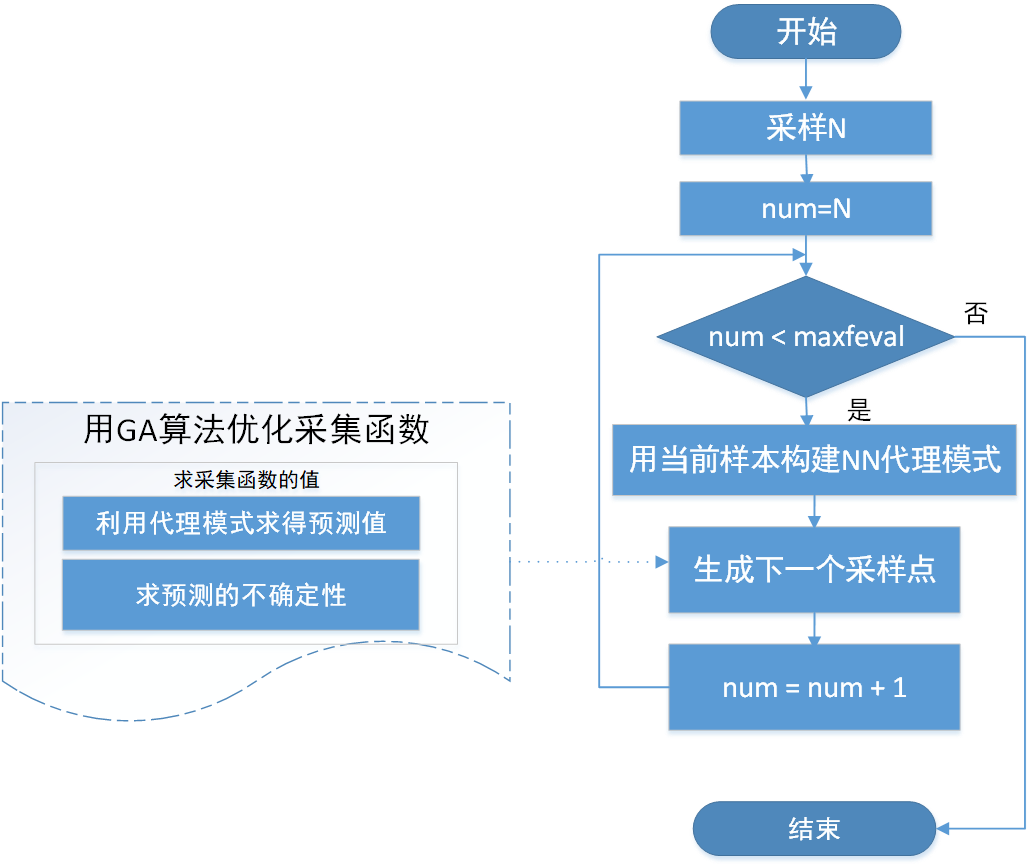
\includegraphics[scale=0.6]{ANN_Kriging流程图.png}
%  \caption{ANNKriging流程图}
%  \label{fig:xfig1}
%\end{figure}
综合前文所述,当前最常用的单目标算法在处理复杂气候系统模式参数优化中面临的主要问题有以下几点:

1.进化算法的种群更新策略慢,优化迭代步数多。在复杂的气候系统模式上进行参数优化是一件高代价的事情,如果优化算法迭代步数多则意味着更多次的模式运行,更多的计算资源被消耗。

2.基于传统代理模式的优化方法代理精度不足。在传统的代理模式优化中,代理模型的选择通常为统计回归方法,这些方法对复杂多峰的气候系统模式的代理精度不足,这将会导致基于代理模式的最优参数估计不够精准,进一步影响优化算法的精度。

面对以上问题,本节设计了基于多层感知机代理模式的优化方法ANN\_CAND。它的主要思想是:(1)利用传统代理模式优化的快速更新策略,ANN\_CAND在初始采样后每一个最优采样点的选取都需要更新优化策略,以期望实现快速的算法收敛过程;(2)利用神经网络的强回归能力弥补现有代理模型在气候系统模式上的代理精度不足的问题,以实现更高的优化精度。

本文中提出的单目标ANN\_CAND优化方法如算法2所示。重要步骤的详细解释如下。

1.初始采样。初始采样有两个重要的目的。其一是为了初步探索参数空间使得优化算法对参数空间有一个基本的了解。其二是为了初始化代理模式。如引言中所介绍,采样方法有很多,这里选择的拉丁超立方采样,它的思想是在参数空间中分层随机抽样。因为有了分层的策略,采样在参数空间中较为全面,能够将优化算法建立在一个良好的基础上。

2.构建基于多层感知机的代理模式。根据气候系统模式的参数到性能的复杂特性,此算法中选择的建模方法是具有更强非线性表达能力的多层感知机神经网络。它是一种前向的人工神经网络(ANN),可以看成一组输入向量到一组输出向量的映射。它由多个节点层所构成,层与层之间全连接,且除了输入层之外,其他的节点层都是带有非线性激活函数的神经元。多层感知机神经网络在非线性回归上十分受欢迎,研究表明多层感知机是通用的函数逼近器,甚至适合非光滑和分段连续回归问题,且其相对于传统的机器学习算法而言,它具有更高的拟合精度~\cite{selmic2002neural}。

3.通过采集函数获取下一个采样点。采集函数为改进后的CAND策略。其主要思想是构建两组候选采样点集合,第一组为在当前最优点处的随机扰动,第二组为在全参数空间中的随机扰动。然后利用两种评价相结合的方法对所有候选集采样点进行评价。第一种评价方法是利用代理模式对采样点进行估计,估计结果好的,被选取的机会大,第二种评价方式是根据候选集中的采样点与当前已有采样点的距离来衡量的,距离越近,估计的结果越准确。另外为了平衡这两个评价策略,引入了一个权重参数weight,weight的值越大,对当前代理模式预测的信任度越高。两组候选集独立选取,平衡了优化过程中的探索与利用。两种评价方式的综合也更加全面地估计了一个候选采样点可能的结果。

4.在真实的模型上评估新采样点的结果。最后将此CAND策略选出的最优样本点带入真实模型中运行,得到真实的采样结果。这一步在复杂函数中为函数值的计算,在气候系统模式中则为一次模型运行和评估的过程。

5.将新采样点加入样本集,重新拟合代理模式。将这一对结果加入已有样本库,重新构建模型。依此重复,直到算法收敛或者是达到规定的迭代步数。

\floatname{algorithm}{算法}
\renewcommand{\algorithmicrequire}{\textbf{输入:}}
\renewcommand{\algorithmicensure}{\textbf{输出:}}
\begin{algorithm}
        \caption{ANN\_CAND单目标优化方法}
        \begin{algorithmic}[1] %每行显示行号
            \Require 原模型$F$, 待调参数$X$, MLP神经网络$M$,利用率$weight$
            \Ensure 优化参数
            \State $S \gets InitSamples( F, X )$
            \For{$i = 0 \to T$}
                \State $FitMLP(M, S)$
                \State $xnew_i \gets \Call {CandMethod}{X,Y,MLP,weight}$
                \State // 将最优估计样本带入真实问题中求解
                \State $ynew_i \gets F(x_i)$
                \State // 将新样本加入已有样本库
                \State $S \gets S \cup (xnew_i,ynew_i)$
            \EndFor
            \Function{CandMethod}{$X,Y,MLP,weight$}
              \State // 获取当前最优结果对应的$X$
              \State $index \gets argmin(Y)$
              \State $current\_bestX \gets X(index)$ 
              \State // CandPoinSet作为下一个采样点的候选集,分为两组,第一组为在当前最优点$X$附近的扰动,另一组为在$X$全空间内的随机扰动
              \State $CandPointSet \gets [RandPerturbatio(current\_bestX),Xrandom]$
              \State // 利用当前训练好的$MLP$模型预测所有的采样候选集
              \State $CandValueSet \gets MLP.predict(CandPointSet)$
              \State // 计算候选集中的点与当前X的距离
              \State $dis\_metrics(CandPointSet) \gets distance(CandPointSet,X)$
              \State // 关于候选集$X$的评价策略分为两部分,第一部分为$MLP$模型对其的预测值,另外一个部分为其与当前采样点的距离
              \State $metrics \gets weight * CandValueSet + (1-weight) * dis\_metrics(CandPointSet)$
              \State  // 选取上述metrics评价最小的点作为下一个最优采样点
              \State $indict \gets argmin(metrics)$
              \State $CandPoint \gets CandPointSet(indict)$
            \EndFunction
        \end{algorithmic}
\end{algorithm}

%\begin{figure}[H] % use float package if you want it here
%  \centering
%  \includegraphics[scale=0.6]{all_SCAM.png}
%  \caption{SCAM在二维参数的变化下导致的性能变化}
%  \label{fig:xfig1}
%\end{figure} 


%对比传统算法,新算法在理论上有以下几点优势。
\subsection{单目标优化方法性能评估}
 为了验证上述单目标优化方法的有效性,分别在复杂数学函数和单柱大气模式(SCAM)上对各类单目标算法进行了测试。因为在真实的气候系统模式中希望以尽可能少的模式运行次数来确定最优参数,以下评比所遵循的规定是对数学函数的计算次数在200次以内,在单柱大气模式上的模拟次数在400次以内,查看在此范围内各类优化算法的表现情况。其中Kriging\_EI是以Kriging为建模模型,以EI为采集函数的代理模式优化方法。RBF\_CAND是以RBF为建模模型,本文中的CAND方法为采集函数。
 
   1.在复杂函数上的测试
   
     为了尽可能模拟复杂的气候系统模式的特点,在这里选择的测试函数是有多个局部最优解,非线性变化较强的Rastrigin和Schwefel~\cite{pohlheim2007examples}函数。Rastrigin公式表达如下所示,
\begin{equation}
\label{equ:Rasfuc}
f ( \mathbf { x } ) = A n + \sum _ { i = 1 } ^ { n } \left[ x _ { i } ^ { 2 } - A \cos \left( 2 \pi x _ { i } \right) \right]
\end{equation}     
     其中$A = 10$,$x _ { i } \in [ - 5.12,5.12 ]$,它在二维参数情况下的函数值变化如图~\ref{fig:sofunctionspace} (a)所示。
Schwefel函数表达式如下:
\begin{equation}
\label{equ:Rasfuc}
     f ( \mathbf { x } ) = 418.9829 d - \sum _ { i = 1 } ^ { d } x _ { i } \sin \left( \sqrt { \left| x _ { i } \right| } \right)
\end{equation} 
其中$x _ { i } \in [ - 512,512 ]$,它在二维参数情况下的函数值变化如图~\ref{fig:sofunctionspace} (b)所示。

\begin{figure}[H] % use float package if you want it here
  \centering
  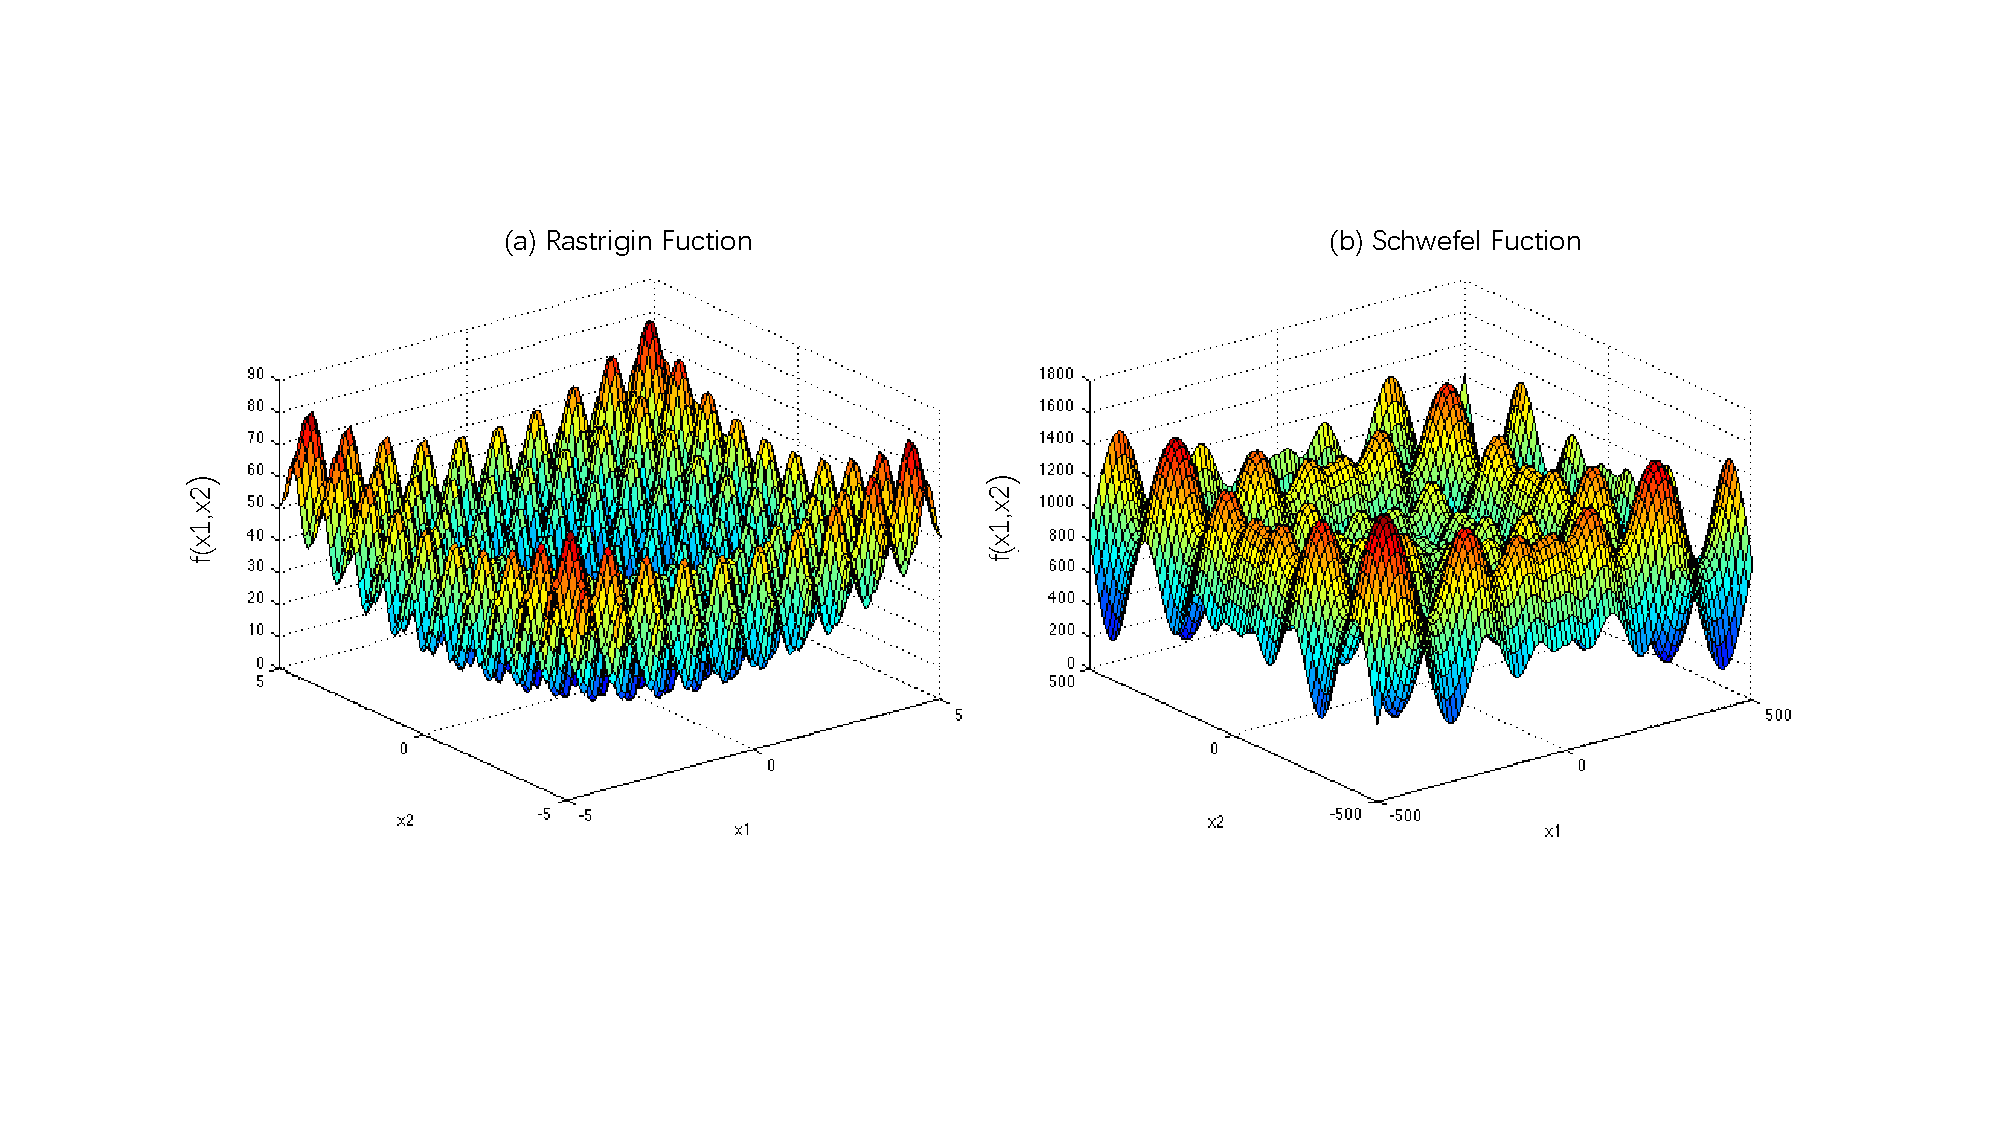
\includegraphics[scale=0.5,trim=10 90 10 100,clip]{figures/fuctionspace.pdf}
  \caption{Rastrigin和Schwefel函数二维空间图(摘自文献~\cite{optfun1,optfun2})}
  \label{fig:sofunctionspace}
\end{figure}

 %   为了验证新算法在参数空间为低维和高维的情况下的性能,这里针对Rastrigin有两组实验,实验1的参数维度为4,实验2的参数维度为12。
 这里将新算法和进化算法以及传统的Kriging和RBF等方法进行比较的结果如图~\ref{fig:sofuction}所示。在Rastrigin和Schwefel函数的优化中基于MLP代理模式的优化算法ANN\_CAND表现较好,和Kriging\_EI,RBF\_CAND一样它相对进化算法能够快速获得较好的优化结果。另外由于选用了更加精准的代理回归方法,它相比于Kriging\_EI和RBF\_CAND而言又能进一步在精度上有所提高。
\begin{figure}[H]
\centering
\begin{minipage}[t]{0.48\textwidth}
\centering
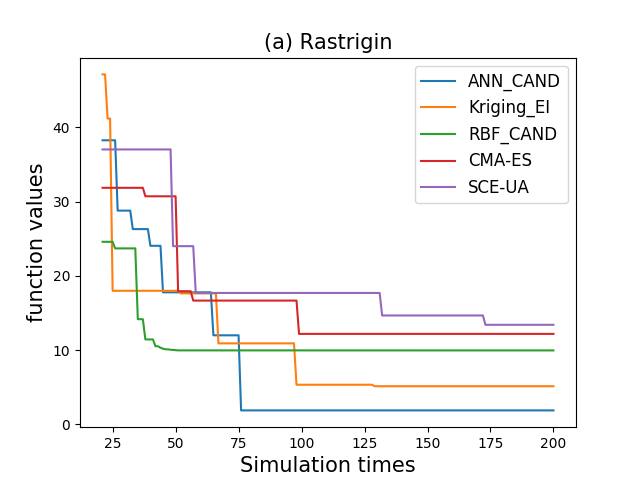
\includegraphics[width=8cm]{figures/all_Ra4.png}
%\caption{ZDT2 hypervolume}
\end{minipage}
\begin{minipage}[t]{0.48\textwidth}
\centering
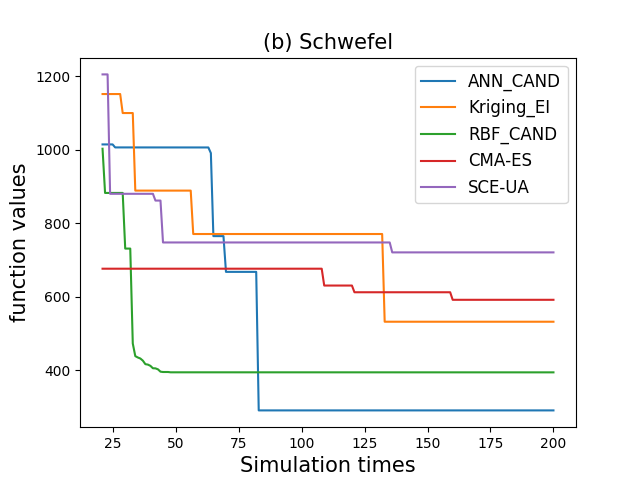
\includegraphics[width=8cm]{figures/all_schw4.png}
%\caption{ZDT2 IGD}
\end{minipage}
\caption{单目标优化算法在Rastrigin和Schwefel函数上的优化结果}
\label{fig:sofuction}
\end{figure}

   2.在单柱大气模式上的测试
   
复杂函数的测试只能证明新算法对于一般复杂的数学问题上的有效性,为了进一步验证其是否能在气候系统模式的不确定性参数调整的实际应用中有较好的表现,本文选择了SCAM( Single Column Atmosphere Model )模式进行测试。SCAM是固定在某个经纬度的单柱大气模式,它是由的特定的边界场和强迫场驱动的,是专门为了研究物理参数化方案而开发的工具,对气候系统模式的发展有重要意义。本文选择的是TWP-ICE~\cite{lin2012twp}和M-PACE~\cite{verlinde2007mixed}实验。TWP-ICE实验的模拟时间是从2006年1月18日至2月13日。M-PACE实验的模拟时间是从2004年10月06日至10月22日。两SCAM个实验性能评价指标是大气模块中最受关注的一些变量,具体的变量选择如表2.1所示。

%%%%table1

%%%%table2
\begin{table}[H]
\centering
\caption{目标变量及其含义}  
\begin{tabular}{ll}
\toprule[1.5pt]
变量名称 & 变量含义 \\  
\hline  
FLUT     & Upwelling longwave flux at top of model   \\
    FSNTOA   & Net solar flux at top of atmosphere   \\
    PRECT    & Total precipitation rate   \\
    Q850     & Specific humidity at 850hPa   \\
\bottomrule[1.5pt]  
\end{tabular}  
\end{table}  
%%%%table3
%\begin{table}[htb]
%\centering
%\caption{相关性分析}  
%\begin{tabular}{llllll}
%\toprule[1.5pt]
%    & FLUT & FSNTOA & PRECT &Q850 &T850 \\  
%\hline  
%FLNT     & 1        & -0.34247 & 0.22897  & 0.03541  & %0.29663 \\
%    FSNT     & -0.34247 & 1        & -0.17576 & -0.18705 & %-0.38863 \\
%    PRECT    & 0.22897  & -0.17576 & 1        & 0.637693 & %0.826208 \\
%    Q850     & 0.03541  & -0.18705 & 0.637693 & 1        & %0.634543 \\
%    T850     & 0.29663  & -0.38863 & 0.826208 & 0.634543 & %1 \\
%\bottomrule[1.5pt]  
%\end{tabular}  
%\end{table}  

     关于如何综合这些变量成为一个评价模式性能的综合目标,本文参考的是文献~\cite{zhang2015automatic}中提出的评价标准。公式如下所示:
\begin{align}
& \left( \sigma _ { \mathrm { m } } ^ { F } \right) ^ { 2 } = \frac{1}{T}\sum _ { i = 1 } ^ { T }  \left( X _ { \mathrm { m } } ^ { F } ( i ) - X _ { \mathrm { o } } ^ { F } ( i ) \right) ^ { 2 }  \label{eq:rel1} \\
& \left( \sigma _ { r } ^ { F } \right) ^ { 2 } = \frac{1}{T}\sum _ { i = 1 } ^ { T }  \left( X _ { r } ^ { F } ( i ) - X _ { \mathrm { o } } ^ { F } ( i ) \right) ^ { 2 }  \label{eq:rel1} \\
& \chi ^ { 2 } = \frac { 1 } { N ^ { F } } \sum _ { F = 1 } ^ { N ^ { F } } \left( \frac { \sigma _ { \mathrm { m } } ^ { F } } { \sigma _ { r } ^ { F } } \right) ^ { 2 }  \label{eq:singleindict}
\end{align}
其中$T$为模拟总时间步,$N ^ { F }$为目标变量的个数。$X _ { \mathrm { m } } ^ { F } ( i )$为模型对于变量$F$在第$i$时间步的模拟结果,$X _ { \mathrm { o } } ^ { F } $为变量$F$在第$i$时间步的观测结果,$X _ { r } ^ { F } ( i ) $为模型对于变量$F$在第$i$时间步的默认实验模拟结果。$\chi ^ { 2 }$越小模式模拟性能越好,如果它小于1,则表明调整参数后的模拟性能比默认实验更优。

不确定参数和取值范围是根据之前的研究来确定的\cite{qian2015parametric,zhang2015automatic}。具体的参数见表2.2,其中zmconv\_c0\_lnd和zmconv\_c0\_ocn是对降水和辐射关系很大的参数~\cite{qian2018parametric},zmconv\_tau是对流降水中最敏感的参数~\cite{yang2013uncertainty},cldsed\_ai也被证明为是对辐射有很强影响的参数~\cite{mitchell2008impact}。
     
\begin{table}[H]
\centering
\caption{待调整的参数及其范围}  
\begin{tabular}{llll}  
\toprule[1.5pt]
\centering
参数名称 & 参数含义 &取值范围  & 默认值 \\  
\hline  
zmconv\_c0\_lnd & Deep convection precipitation efficiency over land & 2.95e-3 ~ 8.85e-3 & 0.0059 \\
    zmconv\_c0\_ocn & Deep convection precipitation efficiency over ocean & 2.25e-2 ~ 6.75e-2 & 0.045 \\
    zmconv\_tau & Timescale for consumption rate deep CAPE & 1800 ~ 5400 & 3600 \\
    cldsed\_ai & Fall speed parameter for cloud ice & 300 ~ 1100 & 700 \\

\bottomrule[1.5pt]  
\end{tabular}
\end{table}  

为了说明SCAM中当前不确定性参数在给定的目标下的调优是否是高峰复杂的优化问题,本文以TWP-ICE为案例,在zmconv\_c0\_lnd和zmconv\_c0\_ocn两维参数空间中进行采样,将每次采样的性能指标(公式~\ref{eq:singleindict})计算出来,得到的空间变化如图~\ref{fig:soscamspace}所示,由图可见,此优化问题十分复杂,非线性很强,适合用来作为气候模式物理参数优化的评价工具。

SCAM上的单目标测试结果如图~\ref{fig:soscam}所示。从图中可以看出在TWP-ICE和M-PACE单柱大气模式上ANN\_CAND算法都表现较好,且在TWP-ICE单柱大气模式中ANN\_CAND相对于其他优化算法的提升更为明显,在M-PACE上Kriging\_EI与ANN\_CAND算法精度表现较为相似。ANN\_CAND优化算法主要是针对复杂、高计算代价的优化问题而提出的,TWP-ICE的模拟时间相对于M-PACE模拟时间较长,模拟的复杂度更高,非线性更强,因此ANN\_CAND在它上的优化效果更为明显。   
\begin{figure}[H] % use float package if you want it here
  \centering
  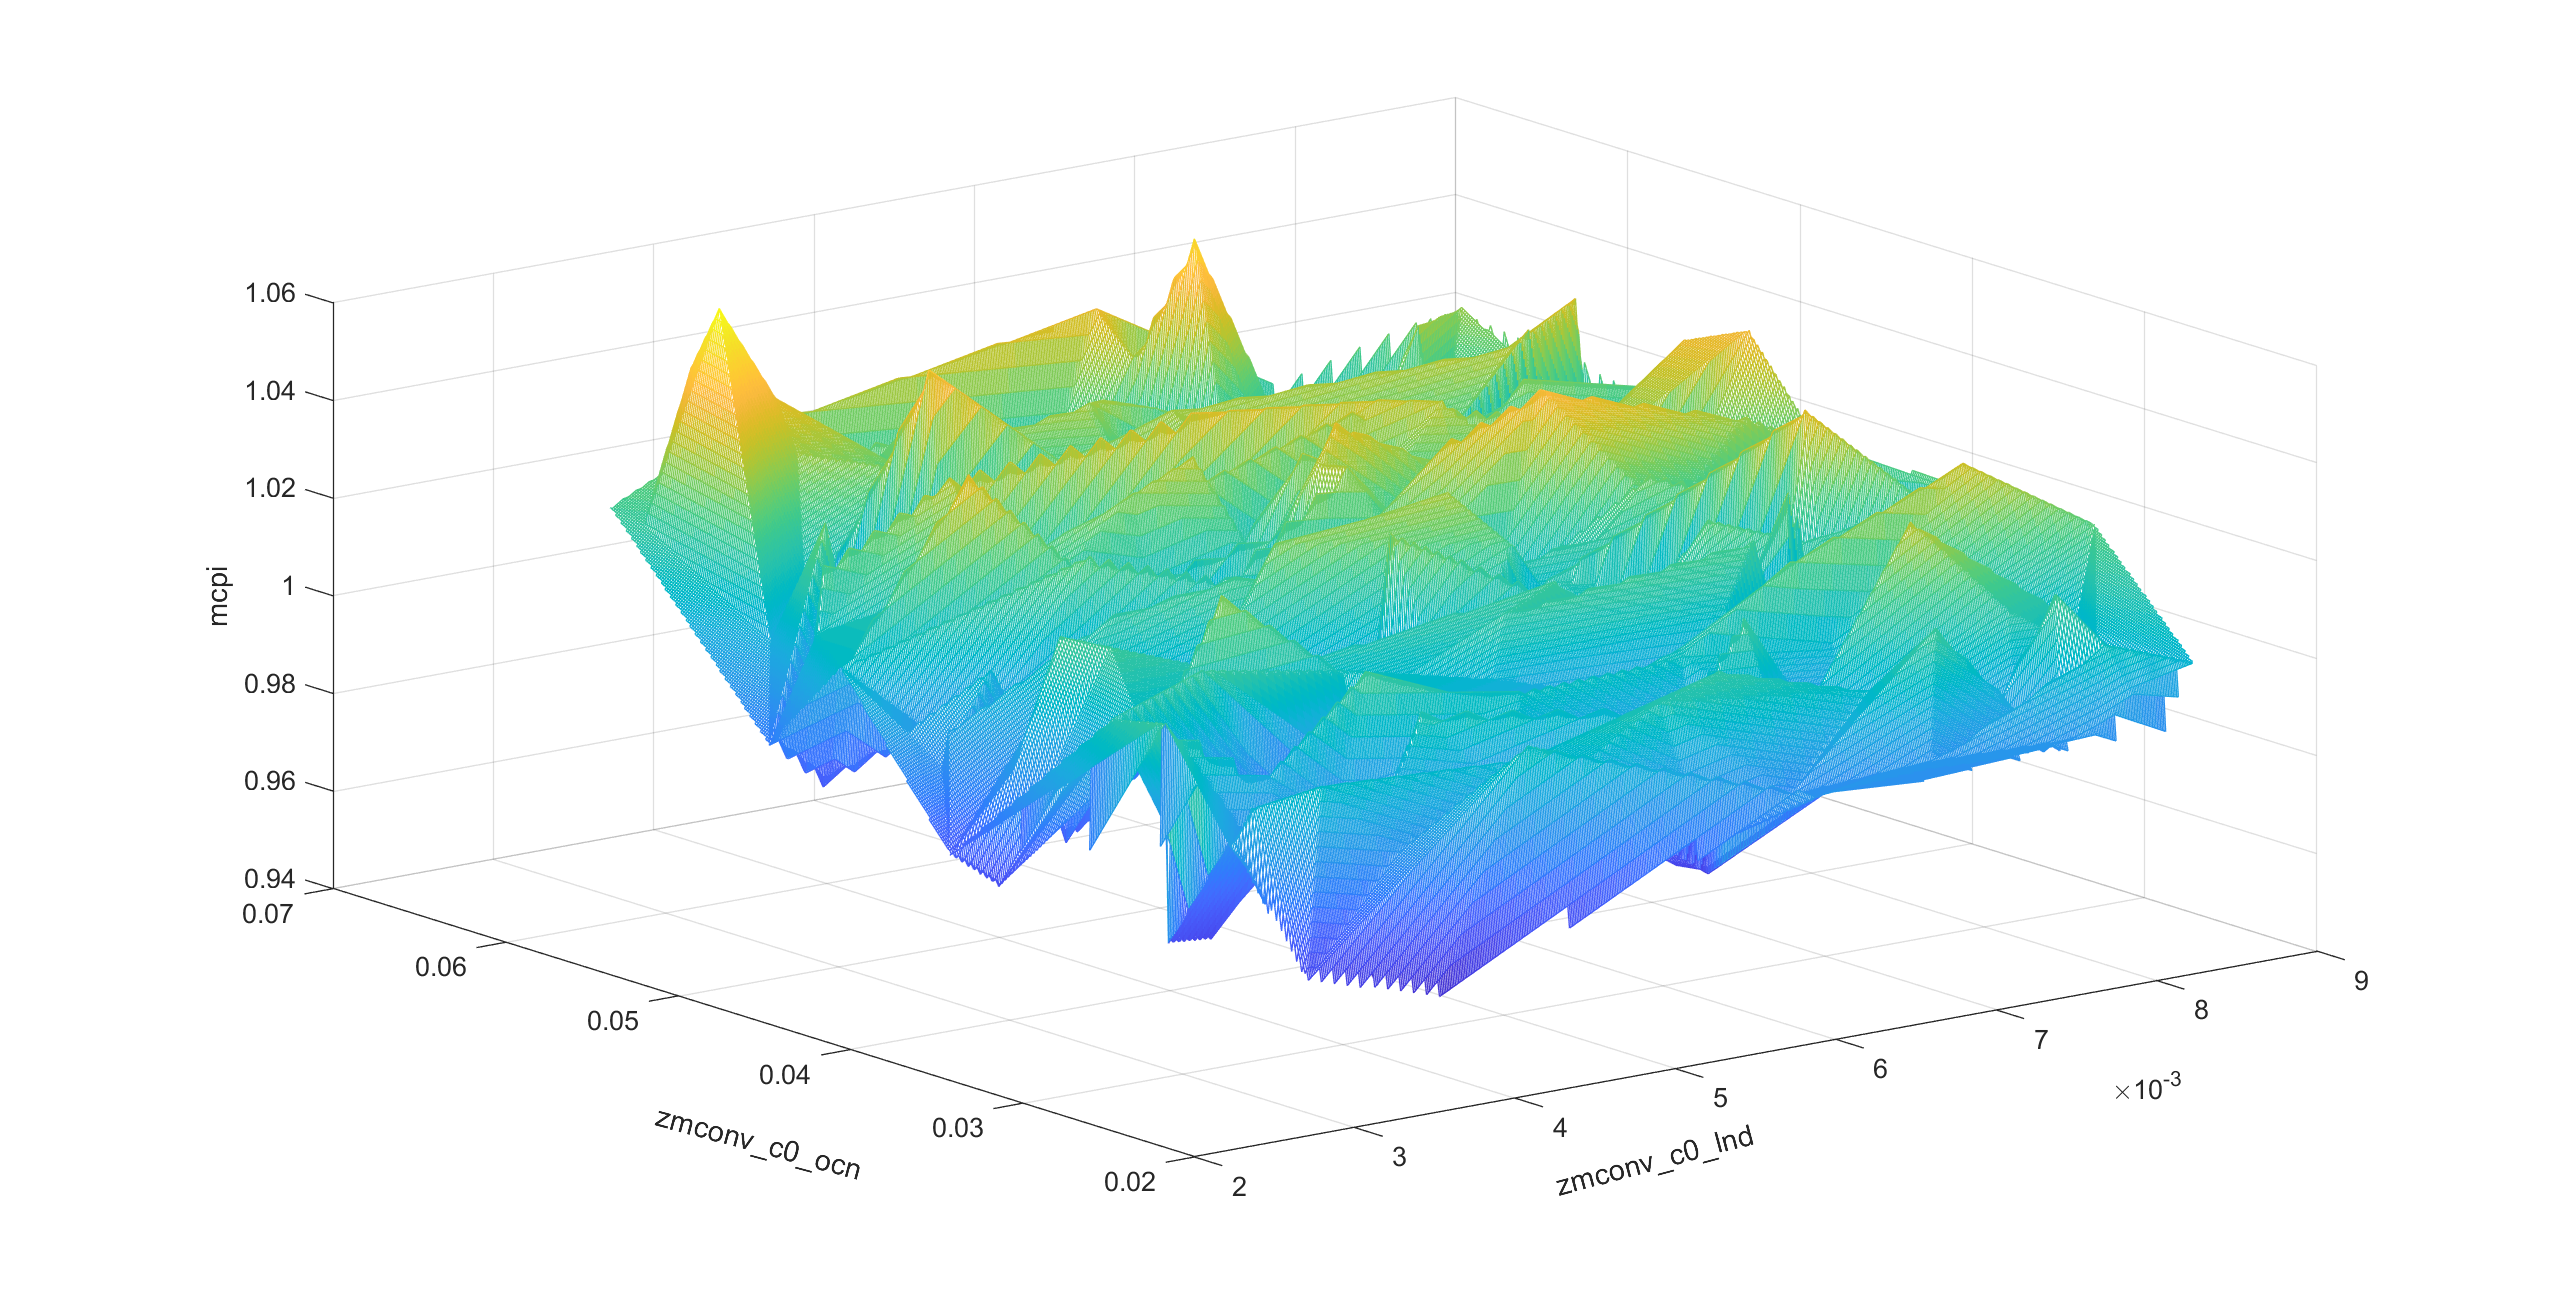
\includegraphics[scale=0.2]{space_SCAM.png}
  \caption{SCAM在二维参数的变化下导致的性能变化}
  \label{fig:soscamspace}
\end{figure}    

\begin{figure}[H]
\centering
\begin{minipage}[t]{0.48\textwidth}
\centering
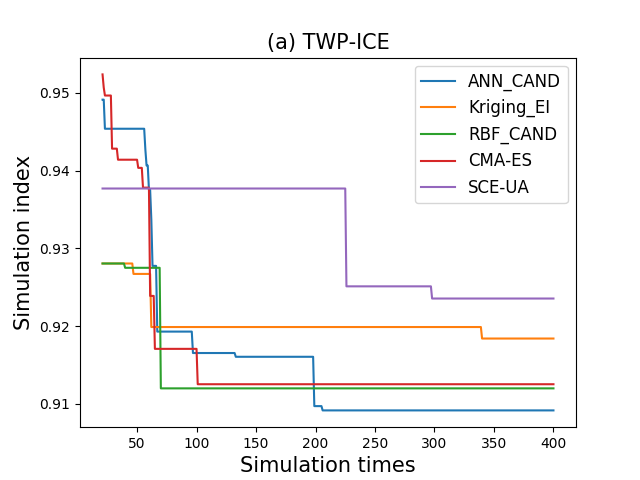
\includegraphics[width=8cm]{figures/twpicescam.png}
%\caption{ZDT2 hypervolume}
\end{minipage}
\begin{minipage}[t]{0.48\textwidth}
\centering
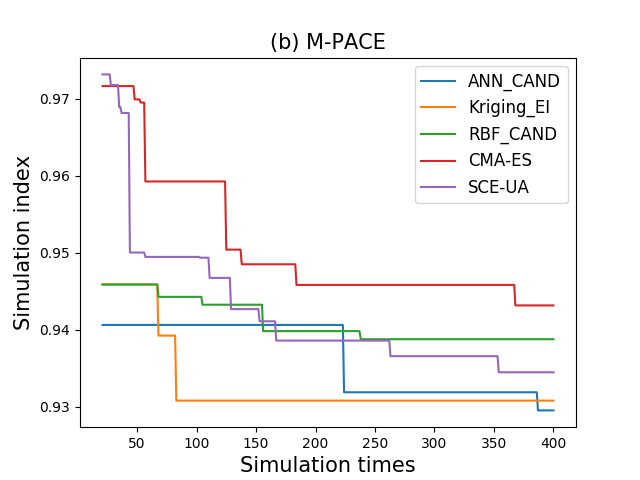
\includegraphics[width=8cm]{figures/mpacescam.png}
%\caption{ZDT2 IGD}
\end{minipage}
\caption{单目标优化算法在TWP-ICE和M-PACE单柱大气模式上的优化结果}
\label{fig:soscam}
\end{figure}

\section{气候系统模式不确定参数的多目标优化方法}
\subsection{多目标优化方法设计}
本文的第一节中叙述了在气候系统模式不确定参数优化中常有多个目标需要同时优化的情况,上文中对单目标代理模式优化和进化算法优化的对比可以看出代理模式优化在复杂问题上大多数情况下都能比进化算法更快地取得相对更好的优化结果,而在Kriging\_EI、RBF\_CAND、ANN\_CAND三个代理模式的评比中本文提出的ANN\_CAND方法在复杂问题中表现较好。在此基础上本小节对上述单目标的ANN\_CAND方法进行扩展,并将扩展后的算法与常见的进化多目标进行对比。另外为了便于下文叙述,在描述多目标优化算法之前,对相关术语进行定义。

定义1 : 非支配解

假设S1,S2为多目标解集中的任意两个点,若对于多目标中的任何一个目标而言,S1的结果都优于S2,则S1支配S2。若S1没有被解集中任何其他的解所支配,则S1为非支配解。

定义2 :  帕累托前沿

帕累托前沿是所有非支配解组成的解集。

多目标优化问题目前最常用的方法是进化多目标算法,例如有NSGAIII (Non-dominated Sorting Genetic Algorithm III)、MOPSO (Multi-objective particle swarm optimization)、MOEA-D (Multi-objective evolutionary algorithm based on decomposition)等算法,其中NSGAIII和MOEA-D算法应用较为广泛。NSGAIII算法是一种带有精英策略的遗传多目标算法,其主要思想是利用hypervolume指标对非支配解进行快速排序,快速获得更全面、更优的非支配解集~\cite{deb2014evolutionary}。MOEA-D算法的主要思想是使用聚合函数将多目标问题转化为多个标量子问题,通过对子问题的优化,不断提高整体优化效果。

面向气候系统模式参数优化,当前多目标算法所存在的问题有:

1.优化迭代步数多。进化多目标算法相比于进化单目标算法,优化收敛性慢,迭代步数多的问题更加显著。从单目标优化问题变成多目标优化问题,所需要的迭代步数是成指数级增长的。

2.基于代理模式的多目标优化算法有待进一步研究。因为传统统计回归方法难以实现高精度的从多个输入向量到多个输出向量之间的回归,所以基于代理模式的多目标优化算法相对欠缺。

%\subsection{多目标优化算法}
本文将ANN\_CAND算法扩展成多目标优化算法(MO-ANN)的伪代码如算法3所示。其主要思想是:(1)应用代理模式优化的思路同时结合进化中多目标优化算法的非支配解排序策略。MO-ANN在每一次寻找当前最优采样点时必须在非支配解中寻找,这样的选择防止选取到的采样点出现一个目标特别好,而另外一个目标极差情况;(2)基于多层感知机神经网络的代理模式能够相对传统的回归方法更好地实现多个输入到多个输出的回归问题。MO-ANN多目标方法的关键步骤解释如下:

1. 非支配解的获取。每一步寻找最优参数将当前所有样本进行比较,找出其中的非支配解。

2. 最优采样点的选择策略。求出非支配解后再对非支配进行排序。非支配解中最好的采样点作为当前已有最优采样点。然后利用文中的扰动方法在已有最优采样点的附近获取更多的候选采样集。

3. 多目标代理模式的应用。多目标代理模式的输入是多维不确定参数,输出为多个目标变量的预测结果。在下一个采样点估计中利用代理模的输出结果和采样点之间的距离为候选集评分。代理模式的多个输出结果的综合如前面在真实采样点中的目标综合方法相同,都默认每个目标的重要程度相当,取多个目标值的平方和再开方。

\floatname{algorithm}{算法}
\renewcommand{\algorithmicrequire}{\textbf{输入:}}
\renewcommand{\algorithmicensure}{\textbf{输出:}}
\begin{algorithm}
        \caption{MO-ANN优化方法}
        \begin{algorithmic}[1] %每行显示行号
            \Require 原模型$F$, 待调参数$X$, MLP神经网络$M$,利用率$weight$
            \Ensure 优化参数
            \State $S \gets InitSamples( F, X )$
            \For{$i = 0 \to T$}
                \State $FitMLP(M, S)$
                \State // 获得当前的非支配解集$X$及其对应的$Y$
                \State Get the current non-dominated solution set $NonDominateX$,$NonDominateY$   
                \State // 利用非支配解集获取下一个最优采样点
                \State $xnew_i \gets \Call {MoCandMethod}{NonDominateX,NonDominateY,MLP,weight}$
                \State $ynew_i \gets F(x_i)$
                \State $S \gets S \cup (xnew_i,ynew_i)$
            \EndFor
            
            \Function{MoCandMethod}{$NDX,NDY,MLP,weight$}
              \State // 将所有的目标综合起来,获取非支配解中最好的$X$
              \For{$i=0 \to nObj$}
                  \State $Y \gets NDY(i)^2 $
              \EndFor
              \State $Y \gets Sqrt(Y)$
              \State $index \gets argmin(Y)$
              \State $current\_bestX \gets X(index)$ 
              \State $CandPointSet \gets [RandPerturbatio(current\_bestX),Xrandom]$
              \State $NobjCandValueSet \gets MLP.predict(CandPointSet)$
              \For{$i=0 \to nObj$}
                  \State $CandValueSet \gets NobjCandValueSet(i)^2 $
              \EndFor 
              \State $dis\_metrics(CandPointSet) \gets distance(CandPointSet,X)$
              \State $metrics \gets weight * CandValueSet + (1-weight) * dis\_metrics(CandPointSet)$
              \State $indict \gets argmin(metrics)$
              \State $CandPoint \gets CandPointSet(indict)$
            \EndFunction
        \end{algorithmic}
\end{algorithm}

多目标的评价标准有很多,例如离散度,世代距离,hpervolume和反世代距离(IGD)等~\cite{riquelme2015performance},其中hypervolume为一个关于非支配解离散度和收敛性的综合指标,因其可以同时考量这两个重要的性能而成为近年来多目标评价指标中最常用的指标之一。IGD指标衡量的是当前获得的假设帕累托前沿与真实的帕累托前沿的距离,是对算法收敛性最好的衡量方法之一,通常hypervolume和IGD配合使用来判断多目标优化方法的优劣。

hypervolume的值为reference point和当前的非支配解围成的超立方体体积,体积越大,说明当前非支配解越接近于真实的帕累托前沿。其公式如下所示:
\begin{equation}
\label{equ:Rasfuc}
H v ( p ) = L e b m \left( \bigcup _ { X \in p } \left[ f _ { 1 } ( X ) , r _ { 1 } \right] \cdot \left[ f _ { 2 } ( X ) , r _ { 2 } \right]  \cdots  \left[ f _ { M } ( X ) , r _ { M } \right] \right)
\end{equation}
其中$M$为多目标的目标个数,$p$为当前获得的近似帕累托前沿,$\left[ f _ { 1 } ( X ) , r _ { 1 } \right] \cdot \left[ f _ { 2 } ( X ) , r _ { 2 } \right]  \cdots  \left[ f _ { M } ( X ) , r _ { M } \right]$为受X支配而不受Reference Point支配的所有点共同围成的超立方体。$Lebm$为勒贝格测度,即在高维空间中的超立方体体积。超立方体体积越大则说明当前获得的近似帕累托前沿与真实的帕累托前沿越相似,优化的效果越明显。

反世代距离评价指标的含义为当前估计的帕累托前沿与真实帕累托前沿的距离,距离越小则说明估计的帕累托前沿越准确。但是在一些复杂的真实应用中,真实的帕累托前沿往往是并不知道的。其公式如下所示。
\begin{equation}
\label{equ:Rasfuc}
\mathrm { IGD ( P , Q ) } = \frac { \sum _ { v \in P } distance ( v , Q ) } { \left| P \right| }
\end{equation}
其中$P$为均匀分布在真实的帕累托前沿上的点,$\left| P \right|$为$P$点集的个数。$Q$为当前算法找到的近似帕累托前沿,$distance ( v , Q )$为$P$中的个体$v$到种群$Q$的欧式距离。

%\begin{figure}[H] % use float package if you want it here
%  \centering
%  \includegraphics[scale=0.6]{all_SCAM.png}
%  \caption{SCAM在二维参数的变化下导致的性能变化}
%  \label{fig:xfig1}
%\end{figure} 
\subsection{多目标优化方法性能评估}
为了评价多目标优化算法的性能和效率,本文将其在ZDT2~\cite{zitzler2000comparison},DTLZ7函数~\cite{deb2002scalable}以及上文提到的SCAM模式上做了以下评测。接下来先简单介绍着两个函数,并叙述了测试结果。

ZDT2优化问题的公式如下所示:
\begin{equation}
\begin{array} { l } { F _ { 1 } = x _ { 1 } } \\ { F _ { 2 } = G ( \vec { x } ) \cdot \left[ 1.0 - \left( x _ { 1 } / G ( \vec { x } ) \right) ^ { 2 } \right] } \\ { G ( \vec { x } ) = 1 + \frac { 9 } { n - 1 } \left( \sum _ { i = 2 } ^ { n } x _ { i } \right) } \\ { 0 \leq x _ { i } \leq 1 , i = 1 , \ldots , n } \end{array}    
\end{equation}

DTLZ7公式如下所示:
\begin{equation}
\begin{aligned} F _ { 1 } ( \vec { x } ) & = x _ { 1 } \\ F _ { 2 } ( \vec { x } ) & = \left( 1 + G ( \vec { x } ) H \left( F _ { 1 } ( \vec { x } ) , G ( \vec { x } ) \right) \right. \\ G ( \vec { x } ) & = 1 + \frac { 9 } { | \vec { x } | } \sum _ { x _ { i } \in \mathbb { T } } x _ { i } \\ H \left( F _ { 1 } ( \vec { x } ) , G ( \vec { x } ) \right) & = M - \frac { F _ { 1 } ( \vec { x } ) } { 1 + G ( \vec { x } ) } \left( 1 + \sin \left( 3 \pi F _ { 1 } ( \vec { x } ) \right) \right) \\ 0 & \leq x _ { i } \leq 1,1 \leq i \leq n \end{aligned}
\end{equation}

多目标问题及其对应的reference point选择如表2.3所示:
\begin{table}[H]
\centering
\caption{多目标优化问题及其reference point选择}  
\begin{tabular}{llll}
\toprule[1.5pt]
样例 & X维度 & 目标维度 & Reference point\\  
\hline  
ZDT2    & 12 & 2 & (11,11)   \\
DTLZ7 & 12 & 3 & (40,40,40)  \\
SCAM & 4 & 4 & (2.5,2.5,2.5,2.5)   \\
\bottomrule[1.5pt]  
\end{tabular}  
\end{table}  

ZDT2,DTLZ7函数的测试结果如图~\ref{fig:mofunctions}。其中NSGAIII和MOEA-D算法的种群数都设置为10,因此图中每一次迭代为10次函数计算。总函数模拟次数也为200次。每10次函数计算之后,进化多目标算法和MO-ANN算法计算一次非支配解的hypervolume和IGD。如前文所述,多目标评价中hypervolume值越大越好,IGD值越小越好,因此本文提出的MO-ANN代理模式多目标优化方法相对于NSGAIII和MOEA-D来说能够更快地提升ZDT2和DTLZ7函数优化效果。
\begin{figure}[H]
\centering
\begin{minipage}[t]{0.48\textwidth}
\centering
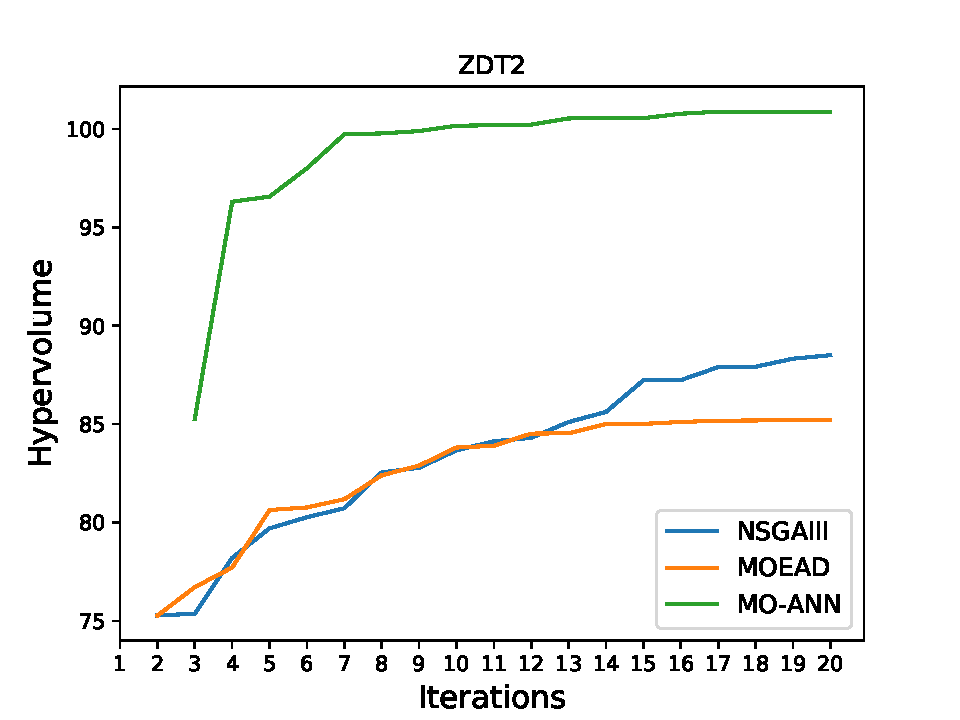
\includegraphics[width=8cm]{figures/hyper_ZDT2.pdf}
%\caption{ZDT2 hypervolume}
\end{minipage}
\begin{minipage}[t]{0.48\textwidth}
\centering
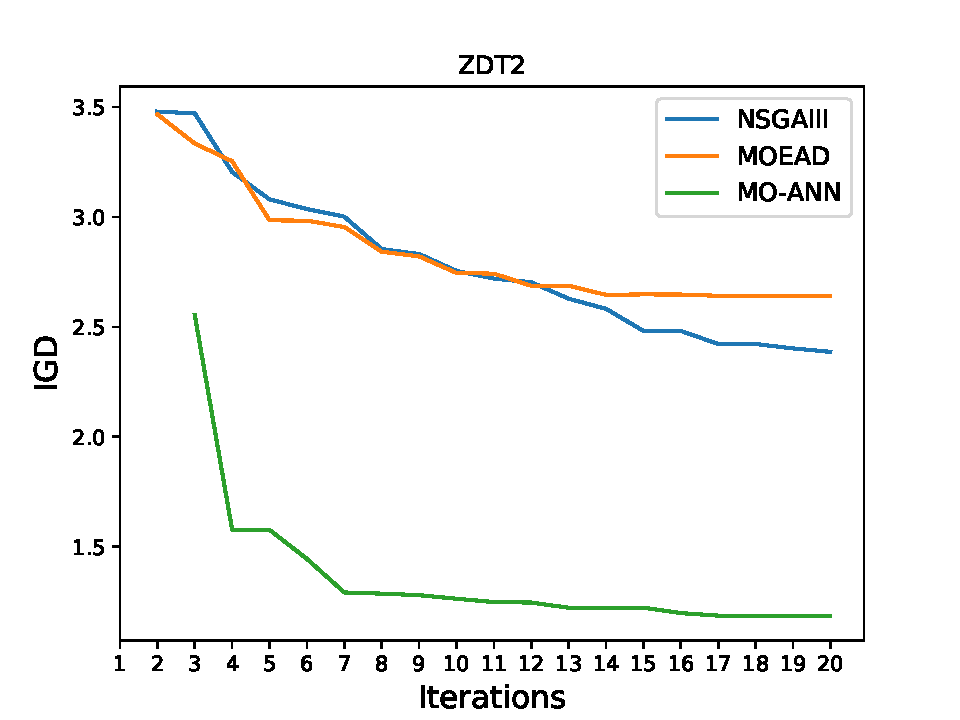
\includegraphics[width=8cm]{figures/igd_ZDT2.pdf}
%\caption{ZDT2 IGD}
\end{minipage}
%\caption{ZDT2函数上多目标优化算法对比}
\\
\centering
\begin{minipage}[t]{0.48\textwidth}
\centering
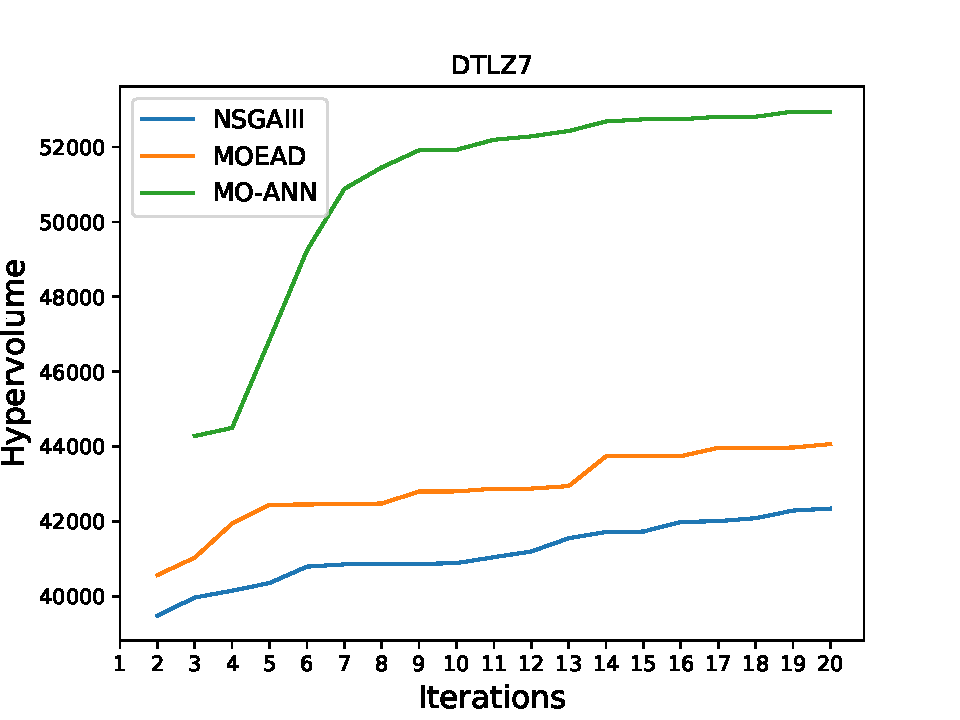
\includegraphics[width=8cm]{figures/hyper_DTLZ7.pdf}
%\caption{DTLZ7 hypervolume}
\end{minipage}
\begin{minipage}[t]{0.48\textwidth}
\centering
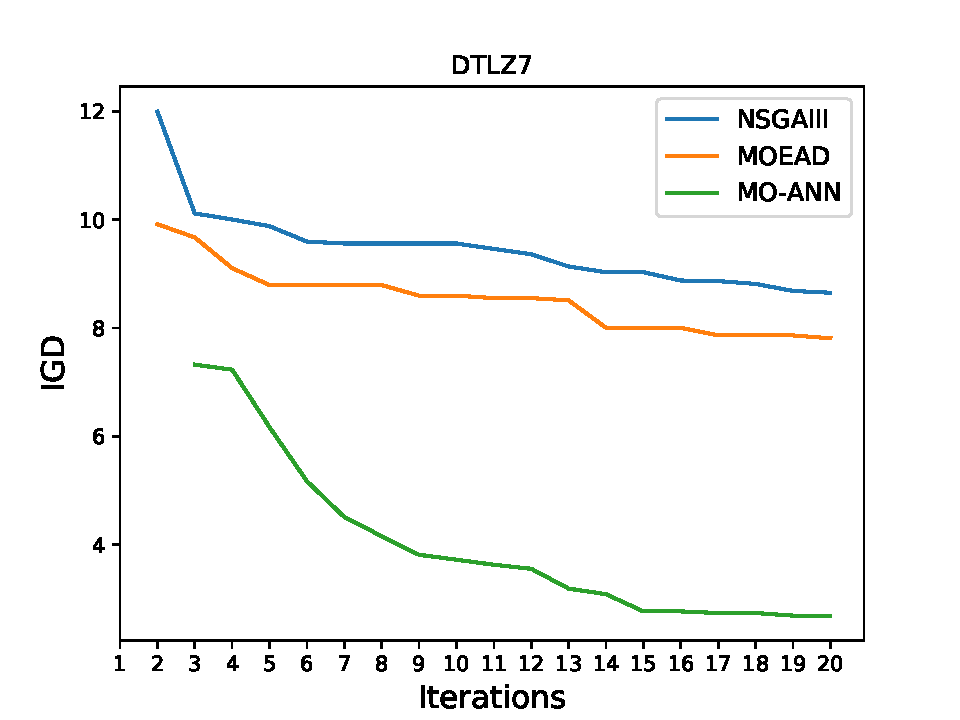
\includegraphics[width=8cm]{figures/igd_DTLZ7.pdf}
%\caption{DTLZ7 IGD}
\end{minipage}
\caption{ZDT2和DTLZ7函数上多目标优化算法对比}
\label{fig:mofunctions}
\end{figure}

为了进一步测试多目标算法在单柱大气模式中的效率,本文接下来将表2.1中的每一个变量的模拟性能作为单独的目标。对表2.2中的不确定参数进行调整,多目标算法评比结果如图~\ref{fig:moscam}。

\begin{figure}[H]
\centering
\begin{minipage}[t]{0.48\textwidth}
\centering
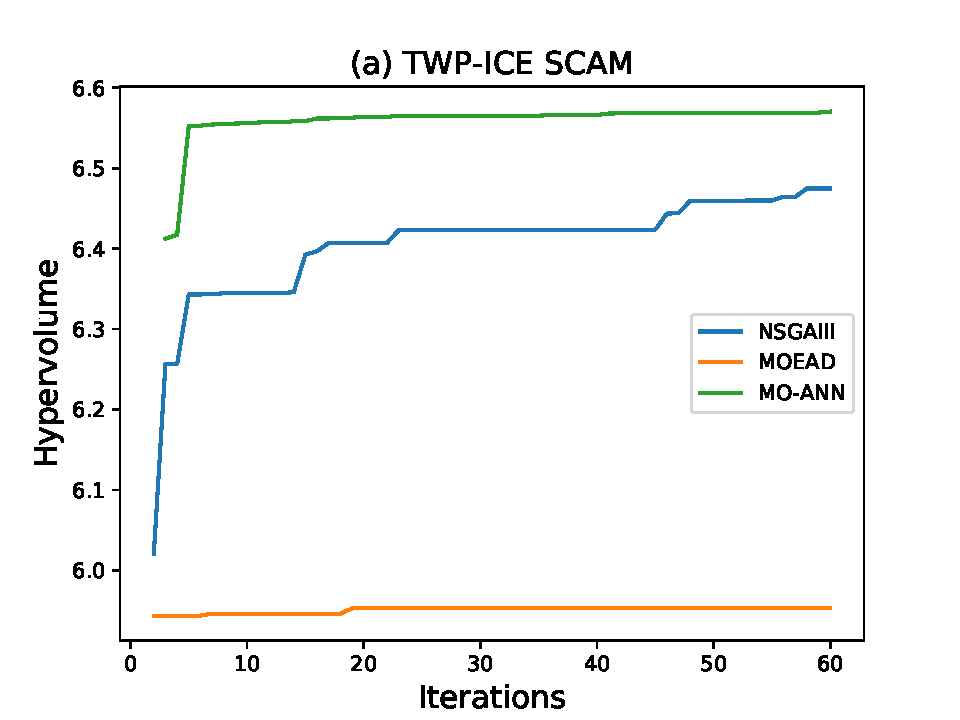
\includegraphics[width=8cm]{figures/MO-TWP.pdf}
%\caption{ZDT2函数上多目标算法的hypervolume}
\end{minipage}
\begin{minipage}[t]{0.48\textwidth}
\centering
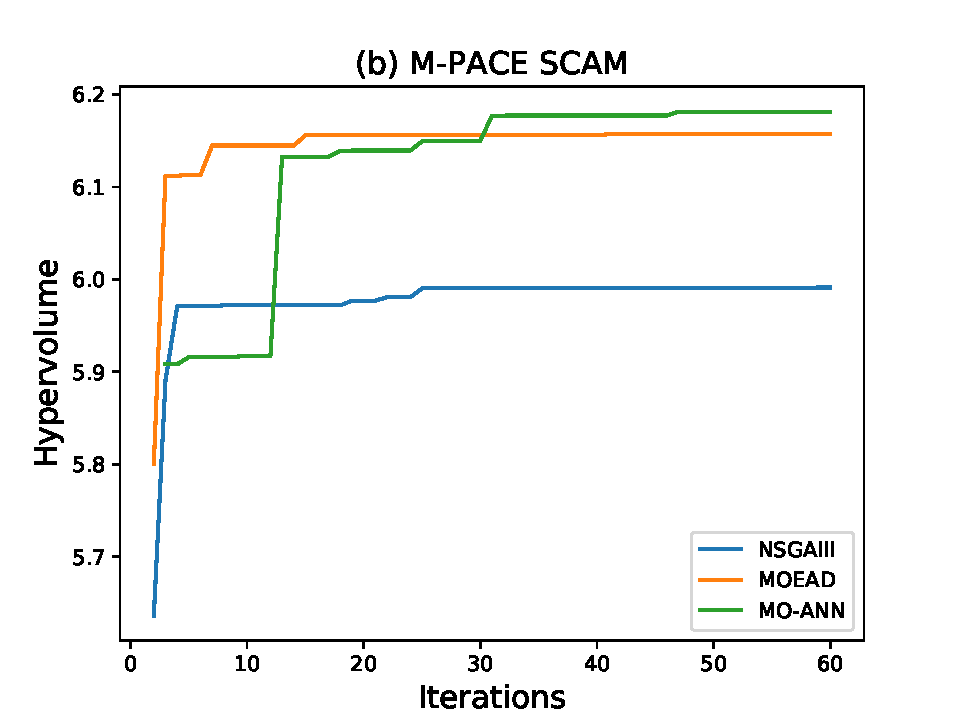
\includegraphics[width=8cm]{figures/ARW-MO.pdf}
%\caption{ZDT2函数上多目标算法的IGD}
\end{minipage}
\caption{TWP-ICE和M-PACE单柱大气模式上多目标优化算法的hypervolume比较}
\label{fig:moscam}
\end{figure}

单柱大气模式无法求出真正的帕累托前沿,因此对于多目标优化算法在SCAM上的评价,本文以hypervolume作为标准。与在ZDT2和DTLZ7上的优化测试相同,这里也将每10次模式运行作为1次迭代,计算一次hypervolume。从图~\ref{fig:moscam}中可以看出在TWP-ICE上MO-ANN能够更快更好地获取更优的非支配解集。在第10次迭代时已经取得较优的结果,而NSGAIII进化多目标算法则优化速度相对缓慢,在第60次迭代时依旧没有完全收敛,MO-ANN收敛速度是它的5倍以上。在M-PACE上的MO-ANN多目标算法的优势虽未能有TWP-ICE上显著,但是也是三个多目标算法中精度最高的算法。

\subsection{基于物理约束的参数优化方法}
如本章第一节中所述,在气候系统模式内有很多物理原理需要遵循,例如大气顶的辐射平衡等,这些物理条件对气候系统模式的模拟性能和模拟稳定性有一定的影响。因此在必要情况下,气候系统模式的参数优化需要考虑物理条件约束的影响。为了使优化算法适应在有约束优化情况下的优化,本节将基于MO-ANN算法进一步设计有约束多目标优化方法。处理有约束优化问题可以分为两大类,第一类是罚函数法,这种方法简单有效,但是针对不同问题,选择合适的罚因子比较困难。第二类方法是将约束问题作为另外一个优化问题,这种方法增加了优化问题的目标,为优化问题带来了一定的难度,但也可以更好的权衡目标和约束之间的关系。

1.罚函数法。罚函数法的思路是如果当前约束得不到满足的话,就将约束乘以一个很大的值加到目标函数上,这样让优化算法记住,此处自变量的选择并不合适。这里根据MO-ANN设计了一个利用罚函数思想的有约束多目标优化算法(MO-ANN-CON-penalty),此算法对于每一个进入代理模式的样本首先计算其约束条件,若约束条件没有满足,则选择一个远大于优化算法因变量的罚因子,将其加到每一个目标变量中。算法的其他部分和MO-ANN保持一致。

2. 约束转化为目标方法。约束转化为目标方法的思路是将约束条件也作为另外一个优化目标。但是在每一次进行非支配排序之前将不满足约束的点从样本中去掉,不让它进入非支配排序。此处的做法也是为了防止迭代在不断进行但是最终没有找到可行解的情况。在对前文MO-ANN算法进行扩展后,转化约束为目标的有约束多目标优化算法(MO-ANN-CON-con2obj)如算法4所示。
重要步骤的解释如下:

(1)可行解进入非支配解排序。每一次在选取当前真实最优采样点时都从当前可行样本中选取非支配解。

(2)目标和约束代理模式的建立。分别为目标和约束构建代理模式,这一点对于气候系统模式的有约束优化问题来说非常重要,因为气候系统模式的约束和输入参数虽关系密切,但并不是一个简单的数学函数表达式,而是一个复杂的经过模式运行和评估所得到的结果,所以为约束也构建代理模式更方便估计输入参数与模式模拟结果之间的关系。


(3)约束转化为目标的最优参数估计。分别用目标代理模式和约束代理模式预测采样候选集中的样本,然后将对应的预测目标和约束组合,然后和前文的MO-ANN一样,选取多目标综合效应好的采样点作为下一个真实采样点。

\floatname{algorithm}{算法}
\renewcommand{\algorithmicrequire}{\textbf{输入:}}
\renewcommand{\algorithmicensure}{\textbf{输出:}}
\begin{algorithm}
        \caption{MO-ANN-CON-con2obj优化方法}
        \begin{algorithmic}[1] %每行显示行号
            \Require 原模型$F$, 待调参数$X$, MLP神经网络$M$,利用率$weight$
            \Ensure 优化参数
            \State $S \gets InitSamples( F, X )$
            \For{$i = 0 \to T$}
            \State //分别为目标和约束建立MLP代理模式
                \State $FitObjMLPModel(M, S)$
                 \State $FitConMLPModel(M, S)$
                 \State Get the non-dominated solution $NonDominateX$,$NonDominateY$ of the feasible solution 
                \State $xnew_i \gets \Call {MoCandConMethod}{NonDominateX,NonDominateY,MLP,weight}$
                \State $ynew_i \gets F(x_i)$
                \State $S \gets S \cup (xnew_i,ynew_i)$
            \EndFor
            \Function{MoCandConMethod}{$NDX,NDY,MLP,weight$}
              \For{$i=0 \to nObj$}
                  \State $Y \gets NDY(i)^2 $
              \EndFor
              \State $Y \gets Sqrt(Y)$
              \State $index \gets argmin(Y)$
              \State $current\_bestX \gets X(index)$ 
              \State $CandPointSet \gets [RandPerturbatio(current\_bestX),Xrandom]$
              \State //利用代理模式估计样本集中的目标和约束
              \State $CandValueSet \gets ObjModel.predict(CandPointSet)$
               \State $CandConSet \gets ConModel.predict(CandPointSet)$
              \State $dis\_metrics(CandPointSet) \gets distance(CandPointSet,X)$
              \State //将约束作为另一个目标,利用代理模式对每个样本集中的样本进行评估
              \State $metrics \gets weight * [CandValueSet$,$Con] + (1-weight) * dis\_metrics(CandPointSet)$
              \State $indict \gets argmin(metrics)$
              \State $CandPoint \gets CandPointSet(indict)$
            \EndFunction
        \end{algorithmic}
\end{algorithm}
\subsection{约束多目标优化方法性能评估}
假设单柱大气模式的模式顶辐射偏差不超过默认实验,辐射偏差的定义为模式顶净短波辐射(FSNT)和净长波辐射(FLNT)之差的绝对值。则上述两种方法在SCAM上的测试结果如下所示。
%\section{自动化的基于ANN代理模式的参数优化平台实现}
\begin{figure}[H]
\centering
\begin{minipage}[t]{0.48\textwidth}
\centering
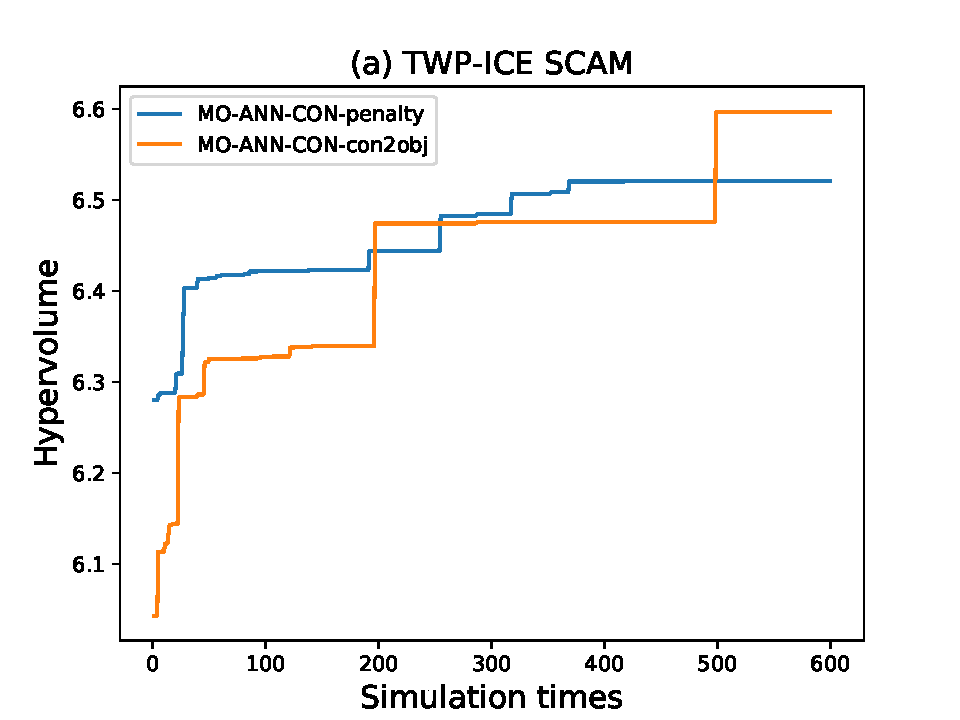
\includegraphics[width=8cm]{figures/twpconstraint.pdf}
%\caption{ZDT2函数上多目标算法的hypervolume}
\end{minipage}
\begin{minipage}[t]{0.48\textwidth}
\centering
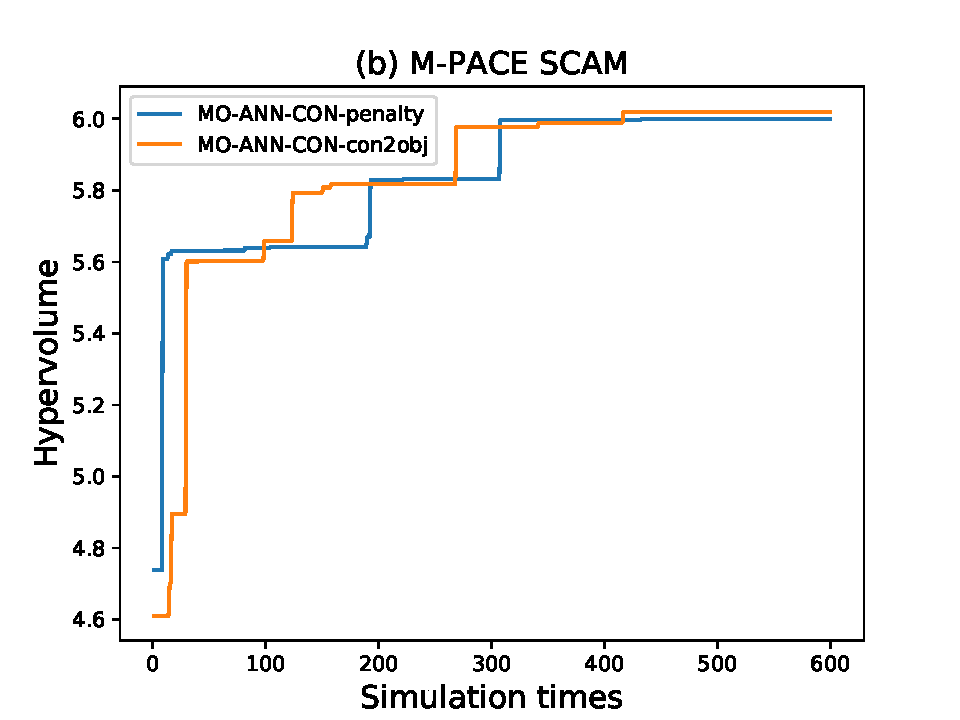
\includegraphics[width=8cm]{figures/constaint3.pdf}
%\caption{ZDT2函数上多目标算法的IGD}
\end{minipage}
\caption{TWP-ICE和M-PACE单柱大气模式上有约束多目标算法的hypervolume比较}
\label{fig:moconscam}
\end{figure}
从图~\ref{fig:moconscam}可以看出在MO-ANN算法上扩展而成的有约束优化算法MO-ANN-CON-penalty和MO-ANN-CON-con2obj在M-PACE上的性能表现较为相似,但是在更复杂的TWP-ICE上,MO-ANN-CON-con2obj方法表现更好。

\section{气候系统模式不确定参数优化方法整合}
前文叙述了在气候系统模式的单目标、多目标以及有约束参数优化情景下,各类基于多层感知机神经网络的代理模式优化方法是如何设计的以及它们与传统代理模式优化以及常用进化算法在复杂数学函数和单柱大气模式上的评估。本节将介绍各类优化算法整合与总体设计。
\begin{figure}[H] % use float package if you want it here
  \centering
  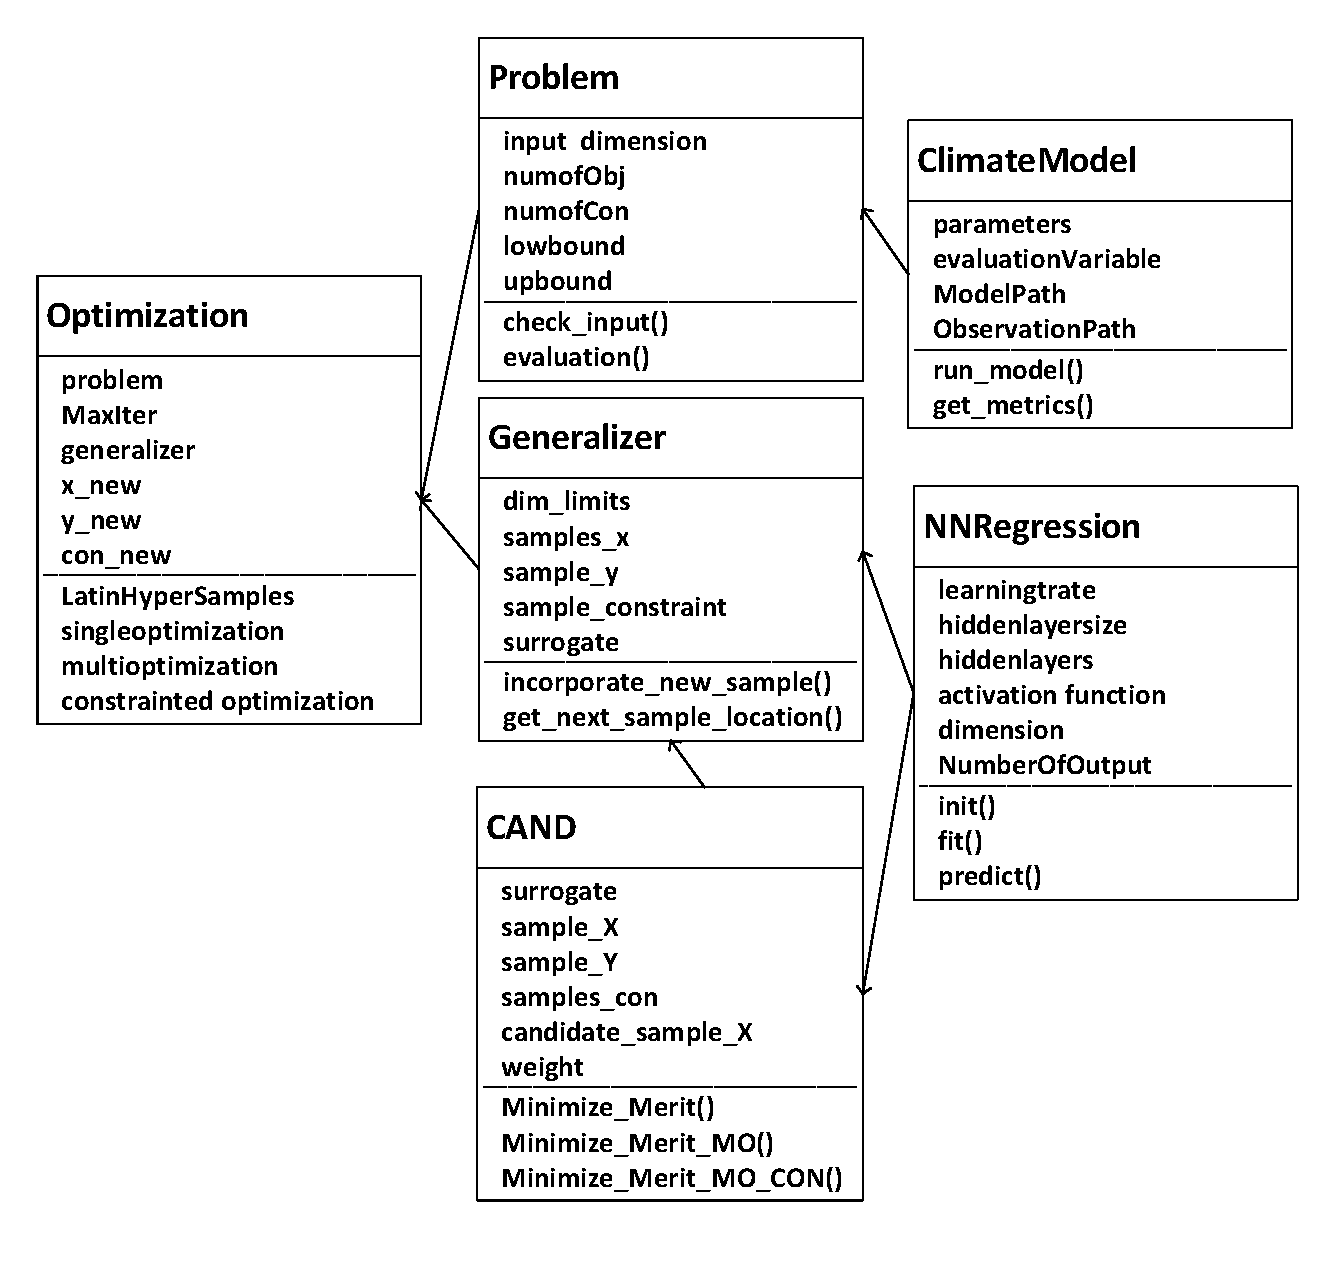
\includegraphics[scale=0.7]{figures/surrogateprocess.pdf}
  \caption{面向气候系统模式的代理模式参数优化方法类图}
  \label{fig:optclass}
\end{figure}   
整合以上单目标、多目标以及有约束优化方法将优化算法通用化,使其能够根据优化场景自动选择合适的优化算法。整合后的优化方法类图如图~\ref{fig:optclass},主要分为以下几个部分。

1.优化总流程的调度(Optimization)。此部分将气候系统模式参数优化的每一个流程串联在一起,包括从一开始的拉丁超立方采样到当前最优采样点的评估,再到下一个真实采样点位置的选取等循环过程,从所选的优化问题可以得出当前是需要单目标优化,多目标优化还是有约束优化,分别选择不同的优化算法对优化问题不断进行探索。

2.优化问题定义部分(Problem)。此部分定义问题的输入维度,输出维度,参数的取值范围,所需要优化问题的评估等,在数学函数上此评估仅为一次函数值的计算,但是对于气候系统模式参数优化来说,这意味着一次模式的运行,模式输出结果的后处理与优化评价标准的获取。在气候系统模式中的一次评估(evaluation)具体步骤有:将当前参数取值匹配到模式中的参数输入文件如namelist中,然后自动启动模式的运行(run\_model),根据优化评价标准设计模式的评估函数(get\_metrics)并获取优化指标的值。

3.通用的代理模式部分(Generalizer)。初始采样所获取的采样点赋值给sample\_x和samples\_y,后续每添加一个采样点都利用incorporate\_new\_sample将其加到已有样本库中。每一个最新样本点的位置都是由它调用优化策略模块(CAND)获取的。它的surrogate部分由NNRegression具体实现。代理模式的fit过程将当前所有样本用来拟合成为一个回归器,代理模式的predict环节利用当前所建立的回归器对未知点进行预测。多层感知机神经网络由输入层,隐含层和输出层共同构成,其中除了输入层之外每一层都带有非线性激活函数,使得模型更能够适应非线性较强的特性表达。特别值得注意的是这里的代理模式的拟合过程,并不是一般机器学习意义上寻求偏差和方差的平衡情况,这里仅仅将其作为一个回归器来使用。所以每一步的拟合过程要尽量准确,和传统代理模式的响应面意义相似。面向气候系统模式物理参数优化的多层感知机代理模式输入为相应的物理参数,输出为多个气候变量的模拟能力,用代理模式来估计物理参数对气候模式模拟性能的影响。

4.优化算法的优化策略部分(CAND)。此部分主要是各个代理模式优化算法的最优样本选择策略。在单目标、多目标、有约束优化的实现过程中有些细节上的调整。估计下一个最优采样点的步骤有:根据当前所有的samples\_x,samples\_y,
samples\_constratint等选取当前真实最优的样本,对此最优样本进行扰动获得待评估参数组合(candidate\_samples\_x),用当前拟合好的代理模式(surrogate)以及离已有样本库的距离对其进行评估。评估结果好的将有机会被带入真正的气候系统模式中进行真实的采样。
   
\section{本章小结}
本章首先分析了气候系统模式中面临的单目标优化、多目标优化以及有约束优化问题,总结了当前各类优化问题分别有哪些常用的算法,对广泛应用的算法进行了简要描述。然后本章对当前优化方法在复杂气候系统模式上使用所存在的问题做了简要分析,并提出了基于多层感知机神经网络(MLP)的代理模式优化算法。此算法利用基于MLP的回归模型代替真实气候系统模式预测最优采样点,每增加一次采样点更新一次代理模型。最后本章将基于MLP代理模式的优化算法与常用优化算法在复杂函数和单柱大气模式上的优化性能进行了对比,并详细叙述了面向气候系统模式参数优化方法的整合与实现。

单目标的ANN\_CAND算法相对CMA-ES和SCE-UA算法来说,它能够实现更快的收敛速度,相对于Kriging\_EI、RBF\_CAND来说,它在精度上有所提升。根据单目标优化算法的评比结果将ANN\_CAND扩展为多目标代理模式优化算法MO-ANN,此方法与当前常用的NSGAIII和MOEA-D算法对比结果表明此方法表现良好,在单柱大气模式上收敛速度最好可相对NSGAIII提升5倍以上。最后为了处理气候系统模式中的物理约束问题,本文将MO-ANN扩展成为基于罚函数和转化约束为目标的约束优化方法,两个方法在单柱大气模式上的比较结果表明转化约束为目标的方法在复杂优化场景精度更高。

综上所述基于多层感知机代理模式的优化算法能够更加全面有效地应对复杂场景的参数优化问题。


%本章的详细结论如下所示:
%(1)单目标优化中CMA-ES算法